
%(BEGIN_QUESTION)
% Copyright 2006, Tony R. Kuphaldt, released under the Creative Commons Attribution License (v 1.0)
% This means you may do almost anything with this work of mine, so long as you give me proper credit

En operatør ber deg (instrumentteknikeren) komme bort og se på en mottakstank for væske. Hun sier at tanken er tom, slik nivåglasset (LG) på siden av tanken viser. Dette er et problem, fordi nivåreguleringssystemet skal holde væskenivået på halv høyde (50\% full):

$$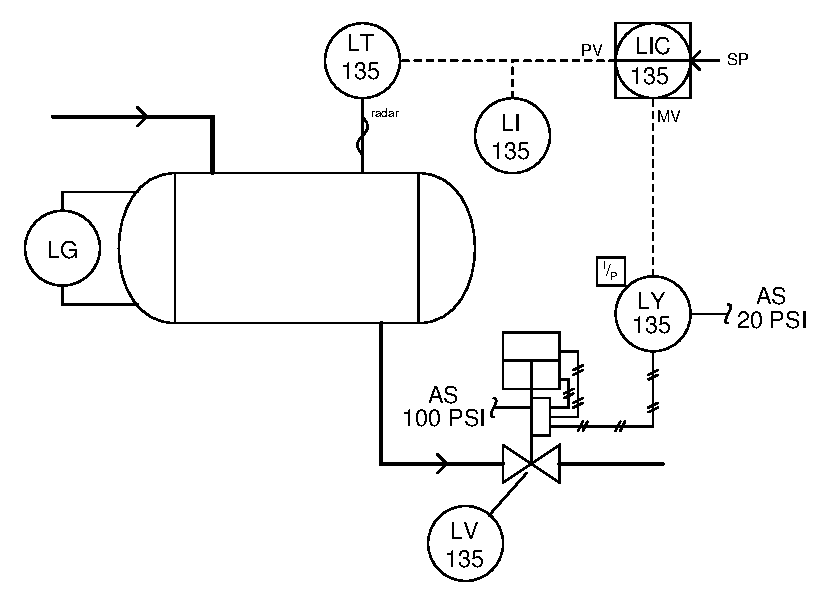
\includegraphics[width=15.5cm]{i01492x01.eps}$$

Det første du gjør er å se på posisjonen til reguleringsventilen, fordi den sitter veldig nær nivåglasset der du og operatøren står. Du ser at reguleringsventilen står helt åpen.

\vskip 10pt

Dette er ikke et nytt reguleringssystem. Faktisk fungerte det helt fint for noen dager siden. Oppgi to ulike instrumentfeil som kan forårsake dette problemet, og forklar {\it hvorfor} hver av disse feilene vil føre til denne situasjonen.

\vfil

\underbar{file i01492}
\eject
%(END_QUESTION)





%(BEGIN_ANSWER)

Dette er en vurderingsoppgave -- ingen svar eller hint oppgis!

%(END_ANSWER)





%(BEGIN_NOTES)

Hvis vi stoler på nivåglasset (selv om slike også kan feile!) som viser at nivået i tanken er altfor lavt, kan vi konkludere med at reguleringsventilen {\it ikke} burde stå helt åpen slik den gjør. Enten blir ventilen (feilaktig) kommandert til å åpne helt, eller så har den feilet åpen av en annen grunn.

\vskip 10pt

{\bf Mulige feil inkluderer:}

\begin{itemize}
\item{} Regulatoren står i manuell modus, 100\% utgang. {\it Dette vil åpne ventilen helt, og den vil ikke reagere automatisk på det fallende væskenivået.}
\vskip 10pt
\item{} Transmitter har feilet høyt (forteller regulatoren at tanken er helt full). {\it Dette får regulatoren til å tro at den må tømme væske fra tanken, og den reagerer ved å åpne ventilen helt.}
\vskip 10pt
\item{} Regulatorutgangen har feilet med 20+ mA utgang. {\it Dette vil drive ventilen til helt åpen posisjon.}
\vskip 10pt
\item{} Ventilposisjoneren har feilet og tvinger ventilen helt åpen. {\it Dette vil åpne ventilen fullt selv om regulatorutgangen ikke ber om full åpning.}
\vskip 10pt
\item{} Dysen i I/P-transduseren er tett, slik at fulltrykk sendes til ventilposisjoneren. {\it En tett dyse i I/P-en gjør at baktrykket stiger ukontrollert og I/P-utgangen metter høyt selv om elektrisk inngangssignal ikke er høyt.}
\vskip 10pt
\item{} Noen har byttet regulatoren fra direktevirkning til omvendtvirkning. {\it Med en direktevirkende transmitter og en signal-til-åpne-ventil skal regulatoren normalt også være direktevirkende. Hvis regulatoren i stedet settes omvendtvirkende, vil PV mettes i én retning i stedet for å stabilisere seg på settpunkt. Interessant nok kan denne feilen like gjerne gi for høyt nivå (overfylling). Feilen er likevel mindre sannsynlig, fordi den som bytter regulatorens virkemåte vanligvis raskt vil se konsekvensene av feilen. Siden systemet fungerte for få dager siden, er byttet virkemåte mindre sannsynlig.}
\end{itemize}

%INDEX% Basics, control loop troubleshooting: determining cause of control problem
%INDEX% Process: receiver vessel liquid level control (generic)

%(END_NOTES)

